%   Filename    : chapter_4.tex 
\chapter{Preliminary Results/System Prototype}

\begin{figure}[h]                
   \centering                    
   \caption{Login and sign up pages}
   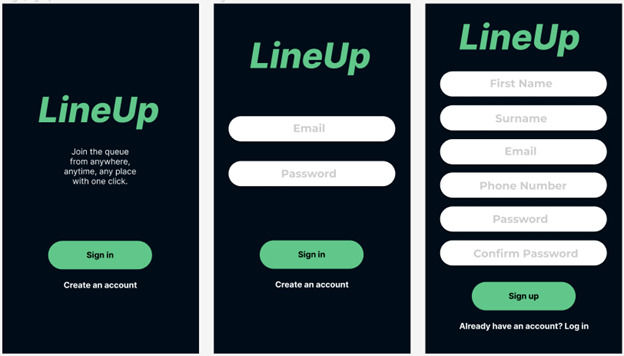
\includegraphics[scale=0.75]{login-signup.png}       
    \label{fig:loginsignup}
\end{figure}

\begin{figure}[h]               
   \centering                    
   \caption{Business account view}
   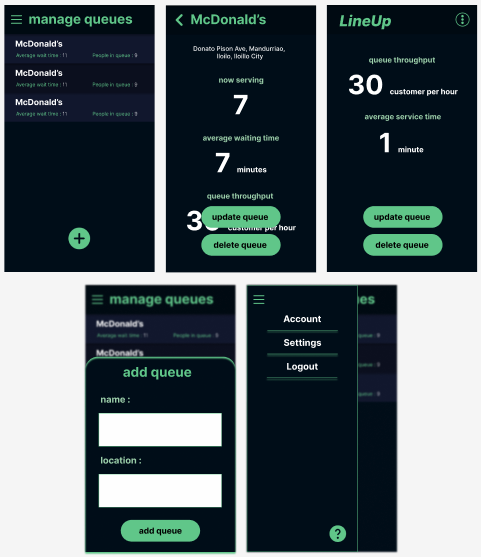
\includegraphics[scale=0.75]{BusinessView.png}       
    \label{fig:businessview}
\end{figure}

\begin{figure}[h]                
   \centering                    
   \caption{Customer account view - Joining Queue}
   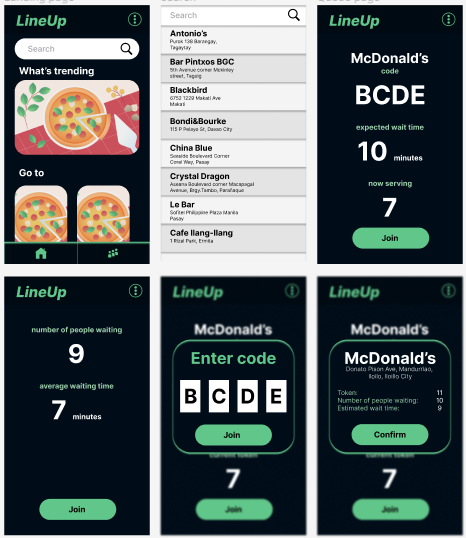
\includegraphics[scale=0.75]{CustomerView1.png}       
    \label{fig:joinqueue}
\end{figure}

\begin{figure}[h]                
   \centering                    
   \caption{Customer account view - Current Queues}
   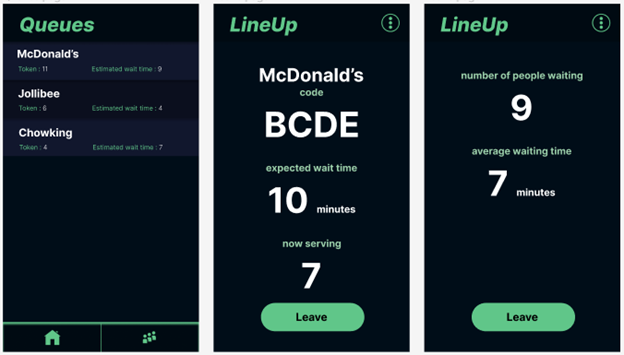
\includegraphics[scale=0.75]{CustomerView2.png}       
    \label{fig:queuecomparison}
\end{figure}

\begin{figure}[h]                
   \centering                    
   \caption{Prompt for your turn}
   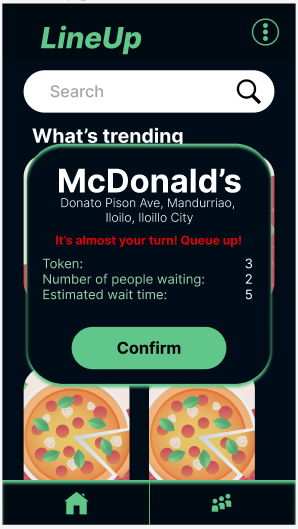
\includegraphics[scale=0.75]{CustomerView3.png}       
    \label{fig:queuenotification}
\end{figure}

\begin{figure}[h]                
   \centering                    
   \caption{Account, settings, and logout screen}
   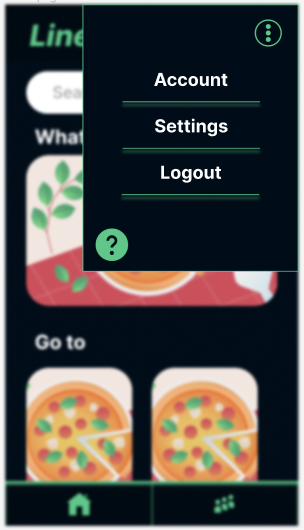
\includegraphics[scale=0.75]{CustomerView4.png}       
    \label{fig:logout}
\end{figure}

Shown here is the project's prototype, which consists of the wireframe for the mobile application. 

As established, the project allows for people to create, manage, and join virtual queues. To facilitate this, there are two types of accounts: \textbf{businesses}, who can create, update, and delete queues for use in their own businesses and services; and \textbf{customers}, who can use the mobile applicaiton to join and exit queues.

As shown in Figure \ref{fig:businessview}, business accounts have a separate view from customer accounts where they are able to manage their queues in a dedicated menu. For each of their queues, an account can view the name of the queue, the number of people currently queueing, and the average waiting time for each queue. They have the option to view a queue in a more detailed menu, where they can access its statistics and manage it further. In this detailed view, they can update a queue, which moves the line forward by one place each time it is tapped.

Seen in Figure \ref{fig:joinqueue}, customers can join a queue through a number of different methods. They may either browse through available queues, or they may enter a code for specific queues. 

Once a customer joins a queue as shown in Figure \ref{fig:queuecomparison}, they are reserved a position on that queue. Using the application, they can view the number of people currently in the queue, the estimated time left for them to wait, and their current position on the queue. When the client’s turn is approaching, the application will send them a notification such as that shown in Figure \ref{fig:queuenotification} so that they may go to receive their service in time. 

At any time, a customer may leave a queue, abandoning their current position on the queue. Alternatively, customers also have the option to delay themselves, moving their position back on the line by a certain number of spaces, with everyone behind them moving forward to take their place. This gives customers more leeway with how long they decide to wait, such as delaying themselves if it is close to their turn but they do not think they can arrive to make their transaction on time.